%%%%%%%%%%%%%%%%%%%%%%%%%%%%%%%%%%%%%%%%%%%%%%%%%%%%%%%%%%%%%%%%%%%
%                                                                 %
%                            CHAPTER FOUR                         %
%                                                                 %
%%%%%%%%%%%%%%%%%%%%%%%%%%%%%%%%%%%%%%%%%%%%%%%%%%%%%%%%%%%%%%%%%%%

\chapter{CHANGE METRICS}\label{ch:graph}

\section{Introduction}

Machine computable change logs provides a very powerful means to begin answering basic versioning questions in a formal and systematic manner.
From the change log, a linked data versioning graph can be extracted and the changes counted to communicate how different are two versions.
The data model was constructed to allow a wide variety of ways to connect together versions such that more complex analytics could be performed using the versioning graphs.
The analytics show that producers must be very transparent when communicating the methods data producers use to assess change impacts as shown in Section \ref{gcmd_85}.

When versioning a data set, researchers very rarely ask whether two objects can be compared.
The data producer often establishes the context in which data objects are sufficiently similar---to use terms from FRBR---\textbf{expressions} of the same \textbf{work}.
Confirming the context prior to making version comparisons is fundamental to ensuring that the resulting versioning graph contains meaningful results.
The data sets described in the following section have sufficient context as established by their producers.
Using the data in these data sets, the model from Chapter \ref{ch:model} is instantiated into versioning graphs.
The graphs are encoded into HTML change logs using RDFa and JSON-LD.
These graphs allow for an analysis of the change between versions, which gives insight into the version identifier.
Finally, a version graph is used to classify the kinds of change separating versions of a data set to determine the utility.

\section{Implementing the Versioning Model}

The following subsections detail the steps used to implement a versioning graph using the model defined in Chapter \ref{ch:model} and the challenges encountered.
Section \ref{mapping} goes through the decisions made to align the attributes within the Noble Gas dataset and within the Copper data set.
The alignments create a formula to detect changes and assign them to either an \textbf{add}, \textbf{invalidate}, or \textbf{modify} change.
A change log can then use the assignments to organize a presentation of the change data.
The underlying versioning graph exists as linked data encoded within the change log, but can also appear as explicit linked data statements.
The linked data uses a custom-made versioning ontology (VersOn) to express the data model using the \textit{vo:} namespace.
The procedure within this section defines the process used to create versioning graphs found in all the following sections of this chapter.

\subsection{Form a Mapping} \label{mapping}

A mapping specifies the method to determine the \textbf{attributes} of a versioning graph and how to compare them.
For spreadsheets and table-based data, row and column indexes initially seem an ideal attribute, but edits often show the contrary.
The Noble Gas data set needed a mapping to align the spreadsheet's columns since 140 columns were removed from the first version.
The remaining columns in the second version no longer had the same column indexes that they did in version 1 so the column headers were used instead.
The Copper data set retains many of the original columns, but their ordering has changed between versions.
In addition, rows must be aligned since both a row and column attribute are necessary to uniquely identify a cell.
The Noble Gas data set split up its rows across eight files, each file representing a separate region of the Earth.
Instead of forming eight versioning graphs or having eight left-hand versions, the files were collected together into a single abstract collection which is then mapped to the right-hand version.
Creating eight versioning graphs would also form eight separate change logs which doesn't make sense since each file forms only a part of the entire work and the second version collects all entries into a single file.
Multiple left-hand versions also doesn't make sense since this creates one change log and graph, but the files are no longer associated with each other.
Cells need to be uniquely identified since this is where a comparison will be made to determine whether a \textbf{modify} change has occurred in a spreadsheet.

Once aligned, determining which attributes have been added, invalidated, or modified is straight-forward.
Attributes which only exist in the original or left-hand version have been invalidated.
More specifically, a set of attributes \(\mathcal{I} = \mathcal{R}_{l} - \mathcal{R}_{r}\) where \(\mathcal{R}_{l}\) and \(\mathcal{R}_{r}\) correspond to the row identifiers of the left-hand and right-hand versions, respectively.
Likewise, a set of attributes \(\mathcal{A} = \mathcal{R}_{r} - \mathcal{R}_{l}\) contain all the added attributes.
Performing the same operations on the columns result in sets of the added and invalidated columns.
A script then iterates over the remaining cells which exist in both versions to determine if they differ, resulting in a \textbf{modify} change.
The unchanged cells form a set of entries which do not appear in a change log or the versioning graph.
The attributes in these sets are then minted into URIs and linked together into the versioning graph, or they can be used to publish a change log.

\subsection{Generate Versioning Graph}

\begin{figure}
	\centering
	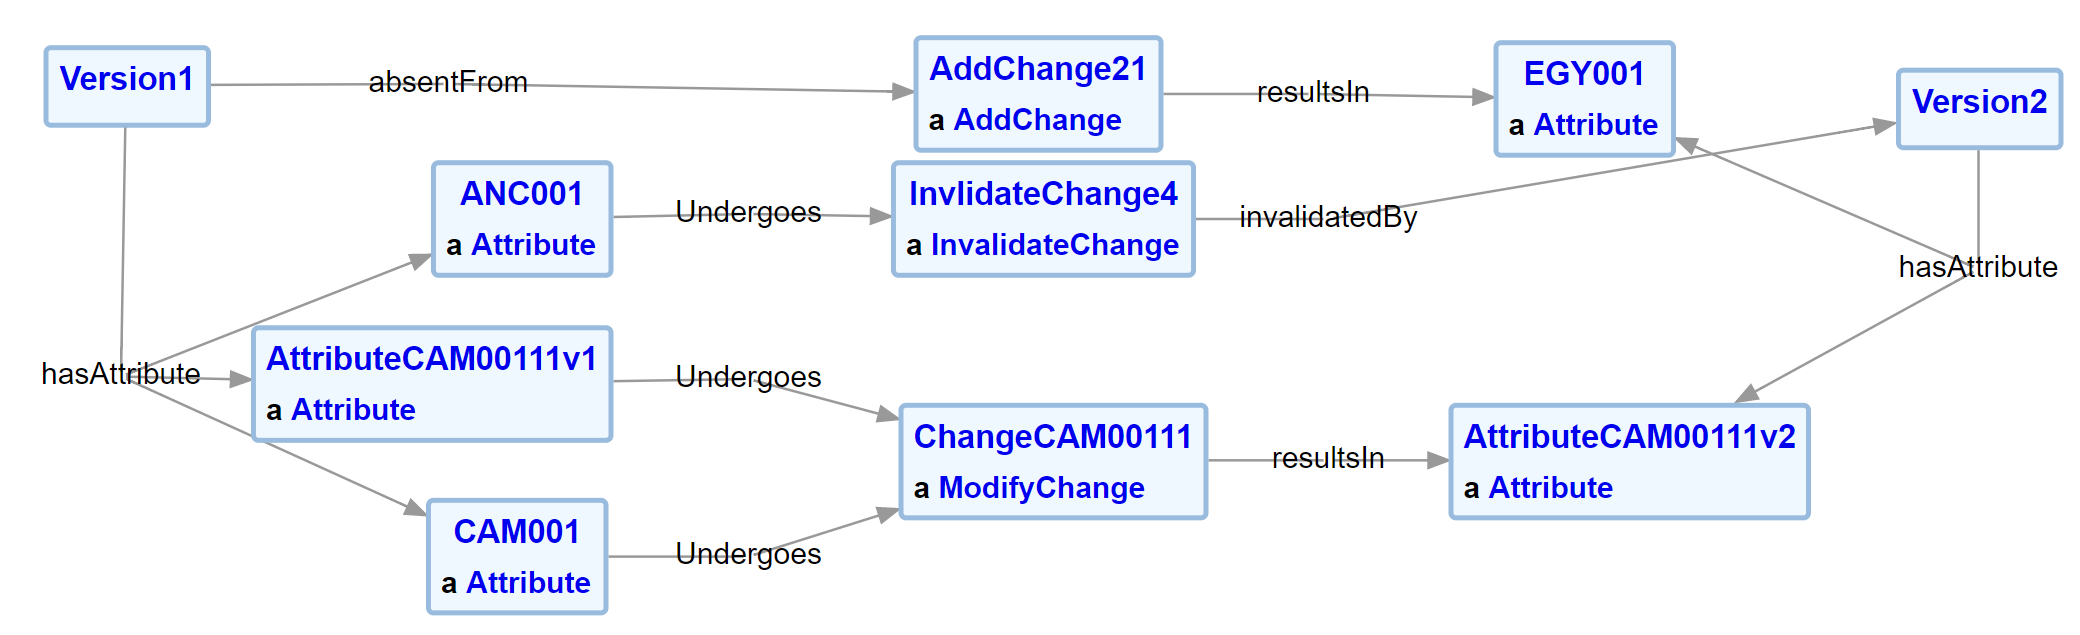
\includegraphics[scale=0.25]{figures/NobleVersion.png}
	\caption{Some initial entries from versions 1 and 2 of the Noble Gas data set}
	\label{NobleGraph1}
\end{figure}
The versioning graphs presented in this section were created by extracting triples from the associated change log which will be covered in Chapter \ref{ch:changelog}.
The statements making up the graph could have alternately been published by writing out the triples directly instead of encoding them into a change log.
Figure \ref{NobleGraph1} displays a subgraph of the Noble Gas data set's versioning graph between versions 1 and 2, highlighting each of the three change operations.
Notice how the versioning graph differs from the provenance graph in Figure \ref{CAM001ProvGraph}.
The versioning graph unpacks the \textit{prov:wasRevisionOf} relationship into explicit components.
These components reveal more detailed differences between version 1 and 2 of CAM001 in the provenance graph which are the differing compilation activities.
\begin{figure}[b]
	\centering
	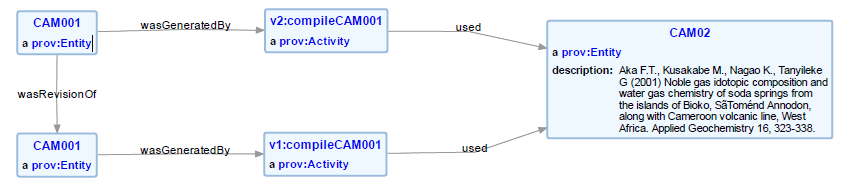
\includegraphics[scale=0.65]{figures/CAM001v1v2.png}
	\caption{Provenance graph for the CAM001 entry of the Noble Gas Database.  Other than the labels, the structure of each data object is very much the same.}
	\label{CAM001ProvGraph}
\end{figure}
The change log encoded the triples in RDFa, resulting in the attribute ``AttributeCAM00111v2" to the right of the \textbf{modify} change.
Because RDFa does not naturally support multiple predicates while also conforming to the content structure of the change log, an attribute was created to combine both the row and column identifier for the changing cell.
Separating the attributes would require multiple dedicated HTML tags which don't appear along with content.
Including these tags would diverge from benefits of encoding triples as attributes.
Figure \ref{NobleGraph1} also shows that even though many columns are added when a new row is added, the row identifier can be used to summarize the columns additions.

Another modification to the implementation differs from the original versioning model.
The \textbf{modify} construction defined in the model only covers the case where a single attribute is sufficient to define a change relation.
The \textbf{modification} captured in spreadsheets describes a cell which requires a row and column identifier to indicate uniquely.
The implementation demonstrates that using multiple attributes is an allowable, sometimes necessary, construction.

Listing \ref{NGA} presents the statements in turtle format necessary to express that the entry EGY001 has been added to the data set from Version 1 to Version 2 as shown along the top of Figure \ref{NobleGraph1}.
The namespace for many of the URIs is \textlangle http://rdfa.info/play/\textrangle.
RDFa allows identifiers to refer to an element on the web page, and the web tool which generated the triples from RDFa, therefore, used its URL as a namespace to produce a valid URI.

\begin{lstlisting}[language=SPARQL, caption=Noble Gas Add in Turtle, label=NGA]
<http://rdfa.info/play/Version1> a vo:Version ;
vo:absentFrom <http://rdfa.info/play/AddChange21> .
<http://rdfa.info/play/AddChange21> a <https://orion.tw.rpi.edu/~blee/VersionOntology.owl#AddChange> ;
vo:resultsIn <http://rdfa.info/play/Attribute21> .
<http://rdfa.info/play/Attribute21> a <https://orion.tw.rpi.edu/~blee/VersionOntology.owl#Attribute> ;
rdfs:label "EGY001"
<http://rdfa.info/play/Version2> a vo:Version ;
vo:hasAttribute <http://rdfa.info/play/Attribute21>
\end{lstlisting}

Figure \ref{CopperGraphVerGraph} shows a similar subgraph from the Copper data set versioning graph.
The graph was assembled using an RDFa change log and also displays a merged attribute on the right side of the \textbf{modify} change.
In the full versioning graph, multiple of each change is present, forming a zipper or ladder-like structure.
As a result, each \textbf{add}, \textbf{invalidate}, or \textbf{modify} change is given separate names for each instantiation.

\begin{figure}
	\centering
	\begin{adjustbox}{addcode={\begin{minipage}{\width}}{
					\caption{Versioning Graph representing the linked data graph with selected entries of additions, invalidations, and modifications. 
			}\end{minipage}},rotate=90,center}
		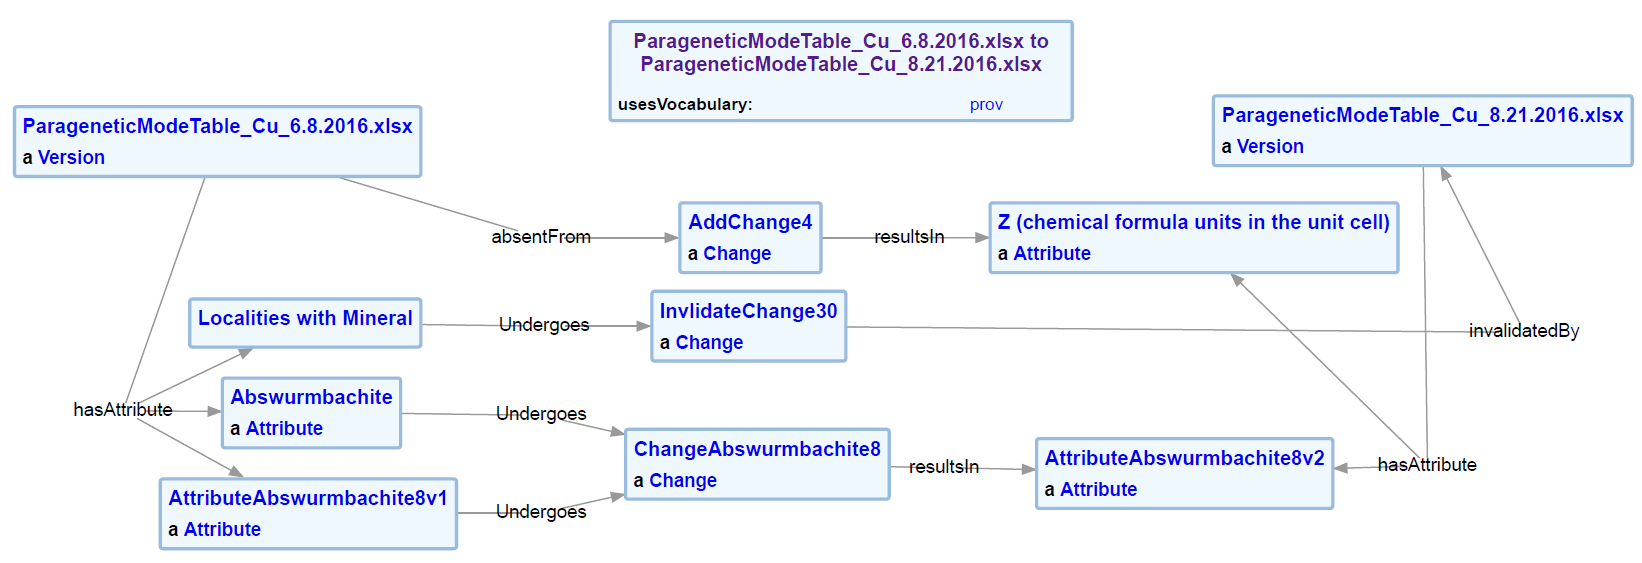
\includegraphics[scale=0.5]{figures/VersioningGraph2.png}%
	\end{adjustbox}
	\label{CopperGraphVerGraph}
\end{figure}

\subsection{Graphs with Multiple Versions}\label{sec:multiver}

Figures \ref{NobleGraph1} and \ref{CopperGraphVerGraph} depict a comparison between only two versions, but a project can contain more than two objects.
Case in point, a third version of the Noble Gas data set was released on July 11, 2017.
Figure \ref{NobleGraph2} shows a subgraph that contains changes from all three versions of the Noble Gas data set.
\begin{figure}
	\centering
	\begin{adjustbox}{addcode={\begin{minipage}{\width}}{
					\caption{Versioning Graph representing the linked data graph with selected entries of additions, invalidations, and modifications after the publication of the third version. 
			}\end{minipage}},rotate=90,center}
		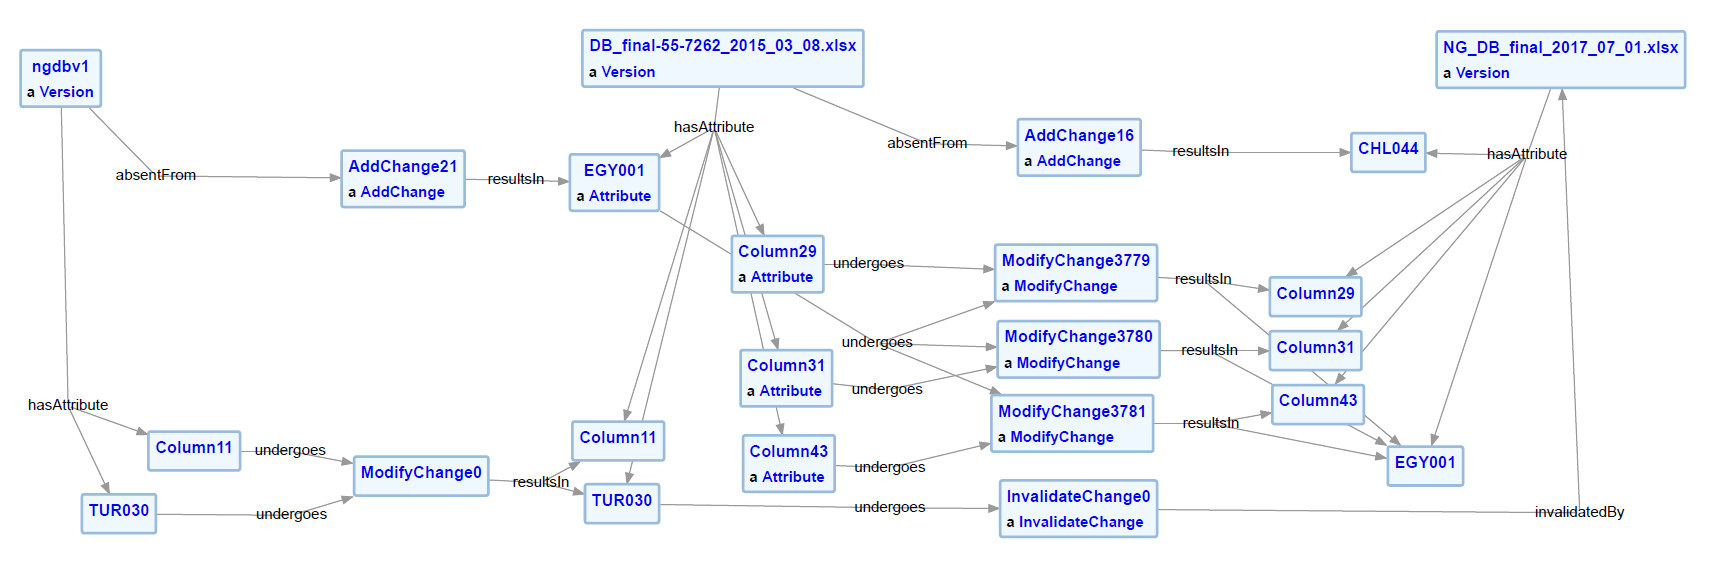
\includegraphics[scale=0.48]{figures/NobleVersion2.png}%
	\end{adjustbox}
	\label{NobleGraph2}
\end{figure}
From the first to second version of the data, EGY001 becomes introduced as an attribute into the data set.
This entry then undergoes a modification change in columns 29, 31, and 43 when comparing versions two and three.
Entry TUR030 goes through a modification change in column 11 from version one to version two.
The entire row, however, becomes invalidated in version three.


Notice the difference in how Figure \ref{NobleGraph1} and Figure \ref{NobleGraph2} refer to columns.
Figure \ref{NobleGraph1} used linked data extracted from a change log employing RDFa, forcing the row identifier and the column identifier into the same concept.
The way nesting works in RDFa means that ChangeCAM00111 cannot back reference multiple concepts in a single statement, therefore AttributeCAM00111v2 was used to imply CAM001.
Figure \ref{NobleGraph2} used linked data extracted from a JSON-LD encoded change log.
Since the log can use explicit statements, the column identifier refers to the entire column and can be used to identify changes in the same column across multiple rows.

\section{Change Metric} \label{ch:distance}

Use Case 2 addresses the use of versions to communicate how different two objects are.
Many versioning systems use dot-decimal identifiers to signify whether a change is large, medium, or small.
The exact requirements to determine change size differs widely across different domains and applications.
The versioning graph provides a new, more regular method to quantify change between objects using versioning operations.
The work done with GCMD Keywords shows the qualitative relationship between version identifiers and change distance.
Work with the MBVL data set then extends VersOn to give more detailed accounting with the change capture method.

\subsection{Utilized Data Sets}

\subsubsection{Global Change Master Directory Keywords}

The Global Change Master Directory (GCMD) is a metadata repository used by NASA to store records of its available data sets \cite{Miled:2001:GCM:372202.372324}.
They employ a set of keywords to make NASA Earth Science data sets searchable.
These words tag and label datasets into strictly defined categories \cite{GCMDKey}.
GCMD Keywords do not qualify as a standard web ontology since it does not constitute a class hierarchy.
The management team stored early versions of the keywords in Excel spreadsheets, and a centralized distribution system was not used until June 12, 2012.
The Key Management Service now serves the keywords directly in a variety of formats.
Each version of the keywords, encoded in RDF, were downloaded into separate files.
Only versions from June 12, 2012 and after were available, resulting in 9 version files.
Each keyword corresponds to a unique identifier, and when combined with a web namespace, resolves to a data description of the keyword.
Every identifier can be referred to per version by including the version's number at the web identifier's end, meaning that identifiers are consistent across versions.
The taxonomy uses the concepts \textit{skos:Broader} and \textit{skos:Narrower}, where skos refers to the Simple Knowledge Organization System ontology name space, to form a tree hierarchy \cite{skos}.
The tree's root is the keyword, "Science Keywords."
The data set provides an interesting study case due its long sequence of versions and ready use of linked data technology \cite{Stevens2016}.

\subsubsection{Marine Biodiversity Virtual Laboratory Classifications} \label{sec:MBVL}

The Marine Biodiversity Virtual Laboratory (MBVL), based at Woods Hole Oceanographic Institution, provides data and services for the study of marine biology with an integrative approach \cite{mbvl}.
In the application studied, a choice of algorithm and taxonomy pairings must be tested on a known population in order to estimate their performance with an unknown microbial population.
The original sequences belong only to the species listed in Table \ref{species_table}.
The original population's census is not available to the author, and only the list of species are known, forming the first data set in this section.
These sequences are then grouped and classified by a specific taxonomy and algorithm pairing.
The workflow utilizes two taxonomies, the Ribosomal Database Project (RDP) and the Silva taxonomy.
Using these databases, the Species-level IdentificatioN of metaGenOmic amplicons (SPINGO) or the Global Alignment for Sequence Taxonomy (GAST) algorithms assign taxonomic ranks to each sequence.
The process produces four data sets, each using the same grouping identifiers and having the same size in each group.
Since the data sets have the same number of sequences, the primary difference between the data sets are the ranks assigned to each sequence.

\begin{table}
	\caption{List of species in the original population.}
	\label{species_table}
	\centering
	\setlength{\tabcolsep}{2pt}
	\begin{tabular}{|c|c|c|}
		\hline
		Acinetobacter baumannii & Actinomyces odontolyticus & Bacillus cereus \\
		Bacteroides vulgatus & Clostridium beijerinckii & Deinococcus radiodurans \\
		Enterococcus faecalis & Escherichia coli & Helicobacter pylori \\
		Lactobacillus gasseri & Listeria monocytogenes & Neisseria meningitidis\\
		Porphyromonas gingivalis & Propionibacterium acnes & Pseudomonas aeruginosa \\
		Rhodobacter sphaeroides & Staphylococcus aureus & Staphylococcus epidermidis\\
		Streptococcus agalactiae & Streptococcus mutans & Streptococcus pneumoniae \\
		\hline
	\end{tabular}
\end{table}

\section{Global Change Master Directory}

\subsection{Global Change Master Directory Versioning Graph}

The Global Change Master Directory establishes the context that each \textbf{manifestation} of their keyword list are related versions.
Since the unique identifier for each keyword remains the same across versions, they can be used to align a mapping across versions.
\textbf{Additions} and \textbf{invalidations} are detected by checking an identifier's presence within both versions.
A \textbf{modification} occurs when a keyword's \textit{skos:Broader} property differs between adjacent versions.
A difference indicates that the word has been moved to a different place within the taxonomy since identifiers do not change across versions and a keyword only has one parent concept.
Changes over consecutive versions can be collected into a single graph using the method in Section \ref{sec:multiver} to chain together versioning graphs.
A change log was generated for each pair of consecutive versions in GCMD Keywords and embedded with JSON-LD.
Versioning graphs for each adjacent version was created by extracting JSON-LD from the corresponding change log, and entering the triples into a Fuseki triple store.

\subsection{Connecting Change Counts to Identifiers} \ref{gcmd_85}

The \textbf{add}, \textbf{invalidate}, and \textbf{modify} counts for each transition are presented in Figure \ref{GCMDC1}.
The query used to extract the counts is found in Listing \ref{gcmd_list}.
Notice the sharp spike in adds and invalidates when transitioning from version 8.4.1 to 8.5.
The version identifiers indicate that at most a minor or technical change has occurred, but the counts of \textbf{addition} and \textbf{invalidation} changes in this transition is more than triple the counts in either of the previous \textbf{major} transitions.
Not only should a small transition not produce changes of this quantity, but the data set's size is on the order magnitude of the recorded \textbf{invalidates}.
In addition, no \textbf{modifications} are revealed, and even the root node "Science Keywords" has been invalidated.
Further investigation of the root word reveals that the name space for the keywords has changed from HTTP to HTTPS.
To provide context, NASA mandated a transition to secure protocols, and the group changed the name space to ensure the URIs remained resolvable.
Since the identifiers are unique, the new name space means they no longer refer to the same object after the protocol change.
Because the keyword identifiers no longer match, the mapping approach results in the total invalidation of keywords from 8.4.1 and the addition of keywords from 8.5.
The dot decimal identifier for the transition from version 8.4.1 to 8.5 does not match the number of changes in the versioning graph.

\begin{table}
	\caption{Global Change Master Directory Keyword Change Counts}
	\label{table:GCMD_main}
	\centering
	\begin{tabular}{|c|c|c|c|c|}
		\hline
		
		Transition&	Add&	Invalidate&	Modify&	Total\\\hline
		June 12, 2012 to 7.0&	310&	9&	22&	341\\
		7.0 to 8.0&	503&	6&	79&	588\\
		8.0 to 8.1&	277&	28&	22&	327\\
		8.1 to 8.2&	53&	1&	26&	80\\
		8.2 to 8.3&	58&	0&	13&	71\\
		8.3 to 8.4&	53&	0&	1&	54\\
		8.4 to 8.4.1&	86&	13&	8&	107\\
		\hline
	\end{tabular}
\end{table}
\begin{figure}[b]
	\centering
	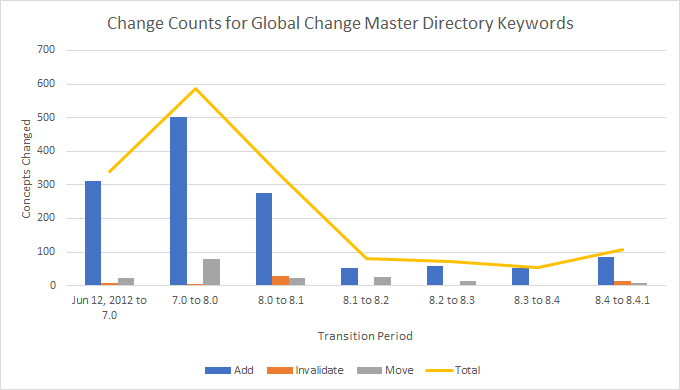
\includegraphics[scale=0.83]{figures/GCMDChartShort.png}
	\caption[Global Change Master Directory Keywords Change counts up to Version 8.4.1]{Add, Invalidate, and Modify counts from the beginning of the Keyword Management System to Version 8.4.1.}
	\label{GCMDC1}
\end{figure}

%\hfill \break
\begin{lstlisting}[language=SPARQL, caption=This query compiles the counts for each subclass of Change in a GCMD versioning graph,label=gcmd_list]
PREFIX vo:<http://orion.tw.rpi.edu/~blee/VersionOntology.owl>
PREFIX rdfs:<http://www.w3.org/2000/01/rdf-schema#>

SELECT ?p (COUNT (DISTINCT ?s) as ?count)
{
?s a ?p .
?p rdfs:subClassOf vo:Change .
} GROUP BY ?p
\end{lstlisting}

Changing the mapping method to account for the new namespace provides a pathway to compare the perceived change by the producer as evidenced by the version identifier with the amount of change in the versioning graph.
To do this, the mapping treats identifiers with HTTP and HTTPS the same. 
Differences in change magnitudes become much clearer after controlling for the altered name space in Figure \ref{GCMDC2}.
All revisions are dominated by \textbf{additions}, but major version changes have counts around 300 to 500 while minor revisions are an order of magnitude smaller.
The transition from version 8.4.1 to 8.5 also seems to follow this trend.
The \textbf{additions} in ``8.4 to 8.4.1" in Figure \ref{GCMDC2} numbers almost a hundred, providing evidence that the trend of decreasing order of magnitudes may now continue as the granularity of the version identifier increases.

\begin{table}
	\caption{Difference in Version 8.5 mapping methods}
	\label{table:GCMD_8_5}
	\centering
	\begin{tabular}{|c|c|c|c|c|}
		\hline
		Mapping Method&	Add&	Invalidate&	Move&	Modify\\ \hline
		Standard&	3097&	3031&	0&	0\\
		Silent&	68&	2&	22&	0\\
		Bridged&	68&	2&	22&	3007\\		
		\hline
	\end{tabular}
\end{table}
\begin{figure}%[b]
	\centering
	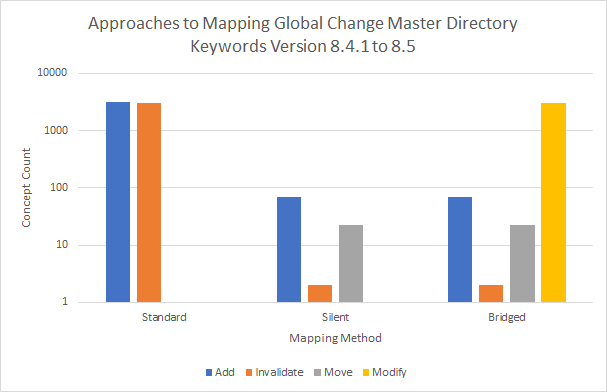
\includegraphics[scale=.9]{figures/GCMD8_5.png}
	\caption{Add, Invalidate, and Modify counts using different methods of mapping identifiers in Global Change Master Directory Keywords Version 8.4.1 to 8.5.}
	\label{GCMDC2}
\end{figure}


\section{Marine Biodiversity Virtual Laboratory}

\subsection{Variant Versioning Graph}

The experiment conducts activity over two phases in this procedure.
The first phase takes sequences from the original known population and feeds the sequences though a particular algorithm/taxonomy combination to produce a candidate classification.
Since the classifications for the known population sequences is unavailable, there is not sufficient context to perform a valid comparison with the candidate classifications.
The second phase compares the performances of each candidate classification of a algorithm/taxonomy pair.
The use of \textbf{add}, \textbf{invalidate}, and \textbf{modify} varies slightly in this application since all the results use the same sequences.
A versioning graph utilizing just the sequence identifiers would only result in \textbf{modify} changes when taxonomic ranks differ since the sequence identifier exists in both data sets.
The mapping instead uses the sequence identifiers to align comparisons and then the taxonomic rank classification to determine the kind of change.
If the right-hand result specifies more taxonomic ranks, the relationship is an \textbf{addition}.
If the left-hand result is more specific, then the relationship is classified as an \textbf{invalidation}.
If both results have the same precision but the name differs, then the link is a \textbf{modification}.
Otherwise, no change is detected.

Figure \ref{mbvl_chart} shows the changes detected when varying either the taxonomy or the classification algorithm.
\begin{figure}
	\centering
	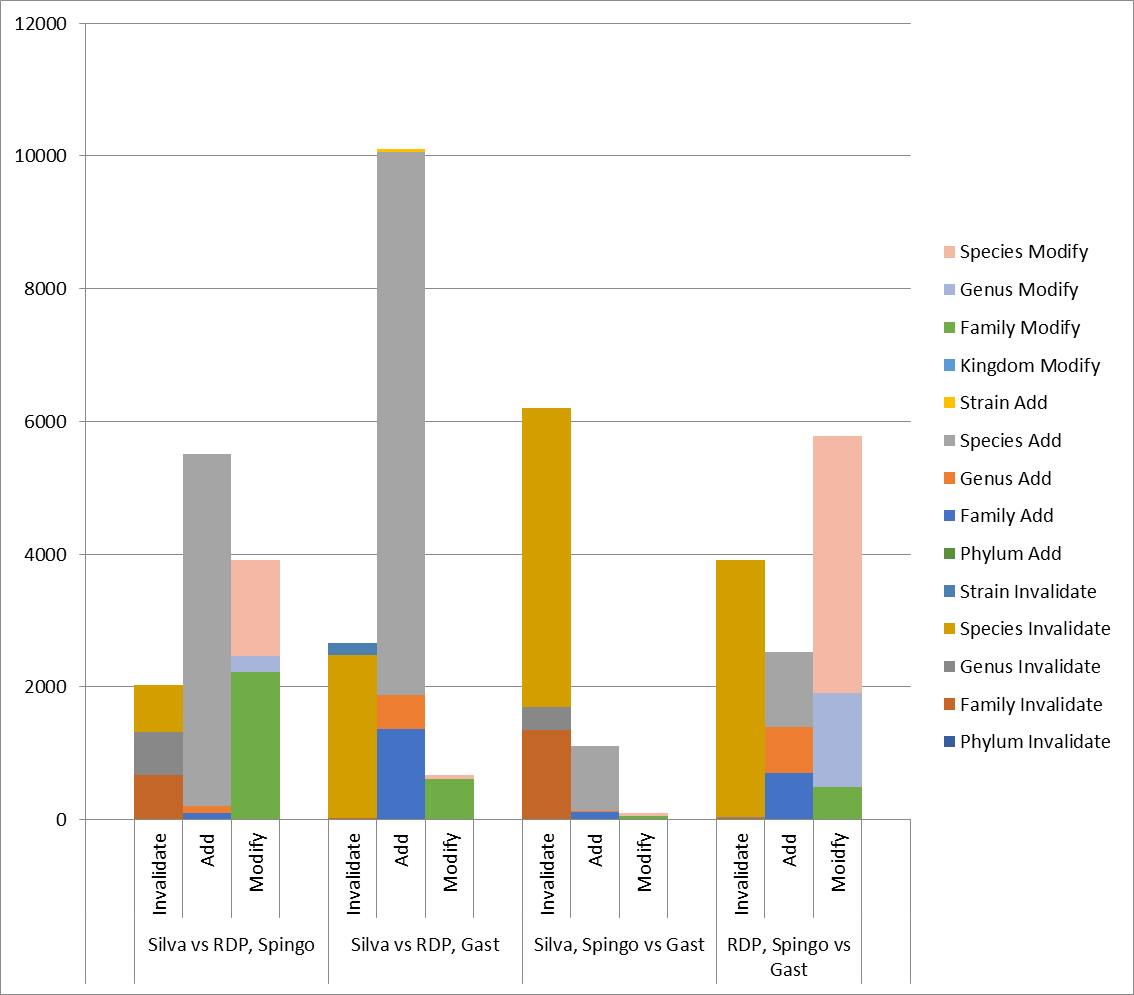
\includegraphics[scale=0.75]{figures/mbvl_chart.png}
	\caption{Compiled counts of \textbf{adds}, \textbf{invalidates}, and \textbf{modifies} grouped by taxonomic rank across algorithm and taxonomy combinations.}
	\label{mbvl_chart}
\end{figure}
No comparison was conducted with different taxonomy and classifier since that would introduce too many sources of variability to differing results in a classification.
Each bar indicates the total number of differences between sequences for a specific kind of change.
The bars are further broken down by the taxonomic rank at which the difference occurred.
For example, in ``Silva vs RDP, Gast", a notable number of classifications differed at the species rank.
The graph also indicates that using the RDP taxonomy often produces more precise classifications since both ``Silva vs RDP, Spingo" and ``Silva vs RDP, Gast" feature a larger number of \textbf{additions} than any other change.
The classifier comparisons feature a high number of \textbf{invalidations}; however, ``RDP, Spingo vs Gast" also displays a higher number of \textbf{modifications} than \textbf{invalidations}.

\section{Version Graph Analysis}

The versioning graph successfully addresses the concerns of Use Case 1 by capturing all the differences within the Noble Gas data set and within the Copper data set into a versioning graph.
Some additional concerns had to be addressed, such as multiple files in a version and dual attribute identification, during the implementation of the versioning model.
The multiple files in the first version of the Noble Gas data set needed to be collected into a single concept in order to preserve the one-to-one relation between versions.
The grouping simplifies the graph structure as well as reduce the complexity of a change log encoding.

In Chapter \ref{ch:model}, there is only one \textbf{attribute} on each side of the interaction.
Figure \ref{CopperGraphVerGraph}, however, shows two \textbf{attributes} used to characterize the \textit{vo:ModifyChange}.
While the model only shows one \textbf{attribute}, it was found that in some applications, multiple \textbf{attributes} may be necessary to properly model a single change.
The construction does not even need to have the same number \textbf{attributes} on both sides of the \textbf{change}.
The flexibility becomes important when trying to model, for example, a single location entry being split into separate latitude and longitude entries.

The version graph's construction allows multiple versions to be linked together.
The graph provides not only greater continuity than Schema.org's properties, but also greater detail than PROV's versioning properties.
Continuity is important since many versioning linked data alternatives view version change as a single contained \textbf{activity}.
When linking together multiple versions using a versioning graph, the relationship between non-adjacent editions becomes implied in the graph's structure.
The natural pathway between \textbf{attributes} in non-adjacent \textbf{versions} holistically considers the relationships among all \textbf{attributes} along that path.
In comparison, other models only capture activity between the adjacent versions.

The model struggles with discontinuous changes to an \textbf{attribute} across multiple versions.
Since the model does not capture when an \textbf{attribute} doesn't change, it is possible for an \textbf{attribute} in an earlier \textbf{version} to become disconnected from later \textbf{versions} due to inactivity.
For example, in Figure \ref{NobleGraph2}, column 31 of EGY001 becomes modified transitioning into the third version.
If that column underwent no activity in the next transition but changed from version four to five, the connection between all the column 31s would no longer be continuous.
This poses a problem for executing queries in a triple store which rely on graph traversals, but no path exists between disconnected \textbf{attributes}.

\subsection{Version Identification}

The versioning process discovered a discrepancy in the identifier assignment in the GCMD Keywords taxonomy.
The original analysis was intended to determine if dot-decimal identifiers could be predicted using the change counts of the versioning graph.
Version 8.5, however, was named with respect to perceived taxonomy changes and did not consider underlying linked data practice revisions.
The disconnect brings into question the accuracy of all prior names and any relationships observed between identifier and change counts.
Non-matching identifiers would explain how 8.4.1 had more additions than any previous minor change but obtains a third bracket identifier.
After accounting for namespace differences in version 8.5, the change counts is in the tens, resembling tallies of other versions in the same identifier bracket.
Version name assignment based on producer perception and not on more concrete measures is concerning.
An incomplete understanding in the amount of change between two versions can lead to flawed expectations during version migration.

The analysis does not to claim that change counts should be the sole mechanism in determining version identifiers.
The counts, however, can provide a more quantitative method to compare version differences.
In Figure \ref{GCMDC2}, the yellow line indicates the total changes made to the data set, performing a similar function as the major/minor/revision version identifier.
Breaking up the changes into types reveals additions dominate manipulations to the data set.
Addition, invalidation, and modification provides deeper insight into how a data set is changing, but some changes can be more impactful than others which this model does not capture.

\subsection{MBVL Analysis}

In Chapter \ref{ch:distance}, the versioning process was used to compare the performance of different taxonomy and algorithm combinations.
The data set diverges from many of the common understandings of versions since each of the versions are not sequential and are largely independent.
The data set of species names in the initial population would not have produced very meaningful results if applied to the versioning model since it lacked sufficient data to map the other data sets together well.

In Figure \ref{mbvl_chart}, the first set of columns in the Silva taxonomy results are versioned against RDP using the SPINGO algorithm.
The naming reflects the orientation in the versioning graph so Silva forms the left-hand version and RDP would be the right-hand version.
In this comparison, using the RDP taxonomy seems to provide more accurate results, most specifically at the species level.
The taxonomies also disagree fairly often at the species and family ranks.
Switching to the GAST algorithm in the second set of columns, RDP once again demonstrates a noticeably greater accuracy in species classification.
There are also significantly fewer disagreements using the GAST algorithm between the two taxonomies.
Looking at the third set of columns, Silva demonstrates greater accuracy classifications under the SPINGO algorithm than under GAST.
Over four thousand of these entries can be classified to the species level when GAST cannot.
In the fourth set of columns, RDP appears to perform better with SPINGO than GAST.
However, the comparison is dominated by a much larger number of disagreements between almost six thousand entries, primarily at the species rank.
On closer inspection, this disagreement is explained by GAST classifying the species for a number of entries as ``uncultured bacterium".
This analysis presents evidence that using the RDP taxonomy with the SPINGO algorithm will produce the most accurate classification results.

\section{Summary}

The results in this chapter implements the versioning model and demonstrates the process and challenges experienced in this endeavor.
The entries in a data set is separated into groups of additions, invalidations, modifications, and unmodified by their attributes.
The grouping occurs over multiple files in the first version of the Noble Gas data set, and the solution was to collect them into a single unit.
The collection keeps the files as one unit, but does not end up addressing other approaches to multi-part versions.

These operational groups organizes the data into a form to publish into a versioning graph.
The approach used to create the graph involves extracting the linked data from a marked up change log.
The decision resulted in constrained representations of the versioning graph, resulting from demands of the encoding methods.
Graphs created using freer form statements, such as the one in Figure \ref{NobleGraph2}, demonstrate an opportunity enable querying over different dimensions of the data.
Changes for specific columns can be queries as easily as individual rows.

The ability to link changes of multiple versions together results as a side effect of the model construction.
Continuously linked changes opens up avenues of exploration to follow change as it propagates through versions.
While change logs will provide a more focused comparison, a triple store with a multi-version graph would give a view of the work through time.
Considering the Noble Gas data set's versioning graph's size, many versions may be difficult to store with large, volatile data sets.

The MBVL data set demonstrates a case where versioning graphs can be used to compare the performance of different taxonomy/algorithm pairings.
The ability derives from sub-classing each of the add, invalidate, and modify changes to give a better perspective where the pairings differed.
This approach of extending the versioning graph adds domain knowledge to the version comparison and helps contextualize the observed differences.
